% ----------------------------------------------------------
% Metodologia
% ----------------------------------------------------------
\chapter{Metodologia}
\label{chap:metodologia}

O trabalho de tese em questão trata-se, essencialmente, do desenvolvimento e testes
de um sistema de \textit{software}. Desse modo, parece desejável, do ponto de vista de
clareza, descrever a metodologia utilizada no trabalho de forma a acompanhar o ciclo
de desenvolvimento dos vários elementos de software utilizados. Para isso, a metodologia
será divida em seções, da seguinte forma:
\begin{enumerate}
\item Termo-hidráulica;
  - Para o gap usar as resistências de contato do Amir (Figura 4.33 + equação abaixo).
  - 4 simulações distintas para o \textit{OpenFoam} para cada potência.
  \subitem Malha;
  - Avaliar a qualidade da malha (ortogonalidade, \textit{skewness},
  suavidade e razão de aspecto).
\item Neutrônica;

  Verificação do milonga com as seções de choque geradas.
  
  \begin{itemize}
  \item Gerar as seções de choque com o Serpent para as condições da tabela 4.35 (a tabela 4.6 é mais consistente) da tese do Amir;
  \item Rodar direto no milonga pra ver o que vai dar (em termos de \textit{$k_{eff}$}).
  \item Rodar a simulação no milonga com os dados interpoláveis artificialmente inseridos para verificar que o esquema consegue interpolar (comparar os \textit{$k_{eff}$}).
  \end{itemize}

  \subitem Geração de seções de choque

  Modelada uma geometria idêntica à representada na malha utilizada pelo \textit{OpenFOAM},
  foram feitas simulações da neutrônica pelo Serpent com objetivo de obter as seções
  de choque em dois grupos a serem usadas na solução da aproximação por difusão dos nêutrons
  pelo \textit{milonga}.

  Na saída do Serpent são dados constantes de groups homogeneizadas (neste caso, com espectro
  corrigido para fugas pelo método B1 \textbf{CITAR}) e outros parâmetros de interesse para
  a modelagem por difusão como, por exemplo, os coeficientes de difusão para cada grupo já
  calculados.

  
\item Acoplamento;
\item Validação.
\end{enumerate}

Como todos os elementos do desenvolvimento estão relacionados entre si, sempre que
julgado oportuno para a clareza do entendimento, os conceitos desenvolvidos em cada
seção poderão ser apresentados conjuntamente. De fato, uma vez que o problema multifísica
(ou acoplamento) nada mais é do que a solução conjunta de dois problemas que são,
usualmente, resolvidos separadamente, é natural como definir, modelar e resolver os
dois problemas separadamente.

De acordo com as definições de problemas acoplados apresentadas
no capítulo \ref{chap:rev}, ao resolver os problemas neutrônico e termo-hidráulico
separadamente, o acoplamento ainda pode ser considerado implícito de acordo com, já que a troca de informações entre os problemas ocorre ao nível de termos completos,
e não em condições de contorno. É importante dizer que essa nomeclatura para as formas
de acoplamento não é unânime na literatura \cite{Ivanov2007}.

Deve estar claro que a metodologia a ser descrita trata do ciclo de desenvolvimento
do \textit{software} acoplado. Apesar de ser possível considerar as simulações e
os processos de pré-processamento e pós-processamento, tanto termo-hidráulicos quanto
neutrônicos, optou-se por tratar destas etapas exclusivamente na seção de validação e,
quando pertinente, nos resultados obtidos.

\begin{figure}[htb]
  \caption{Metodologia: o sistema acoplado.}
  \centering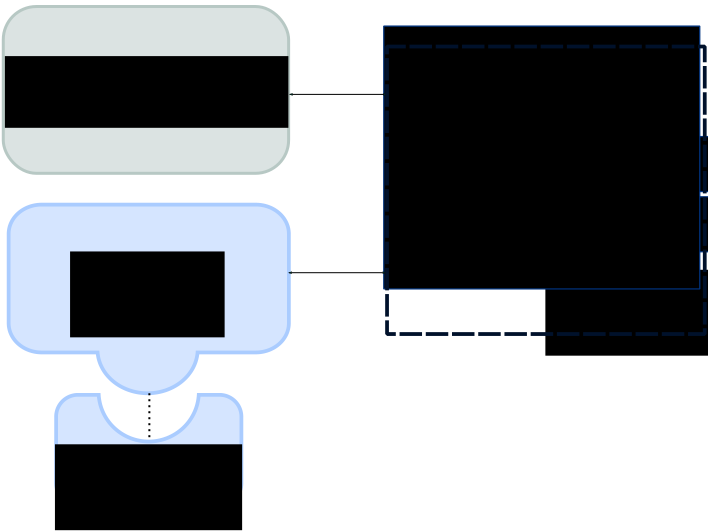
\includegraphics[scale=0.7]{figuras/metodologia1.png}
  \label{metodoetapas}
  \legend{Fonte: autor}
\end{figure}

Na figura \ref{metodoetapas} são apresentadas as relações entre os diferentes elementos
do sistema acoplado.



\section{Termo-hidráulica}
\label{sec:th}

Para a realização dos cálculos termo-hidráulicos, é usado o \textit{software OpenFOAM},
um sistema de \textit{CFD}.

\begin{itemize}
  \item Citar o \textit{perf} como avaliador de desempenho do acoplamento. (citar).
\end{itemize}

\subsection{Geração de Seções de Choque}
\label{sub:xs}

As seções de choque e os parâmetros delas derivados para os cálculos neutrônicos
determinísticos (como o coeficiente de difusão, por exemplo) são gerados pelo
código \textit{Serpent}.
Para isso, foi modelado um quarto de combustível tipo TRIGA.\ref{mini-triga}.

\begin{figure}[htb]
  \caption{Núcleo para geração de seções de choque.}
  \centering\includegraphics[scale=0.7]{figuras/triga-like.png}
  \label{mini-triga}
  \legend{Fonte: autor}
\end{figure}




